\documentclass{beamer}
\usepackage[utf8]{inputenc}
\usepackage[english,russian]{babel}

\usepackage{xcolor}

\usepackage{amsmath,amsfonts,amssymb,amsthm,amscd,amsxtra}
\usepackage{physics}
\usepackage[sharp]{easylist}
\usepackage{comment}
\usepackage{mathtools} % xmapsto, \Vector

\usepackage{beamerthemesplit}
\usetheme{Boadilla}
\setbeamertemplate{caption}[numbered]

% \usepackage[pdftex]{graphicx}
\graphicspath{ {pic/} }
\usepackage{tikz}

\newcommand{\hilb}[1]{\mathcal{H}_{#1}}
\newcommand{\cconj}[1]{\overline{#1}}
\newcommand{\hank}[1]{H_{#1}^{(1)}}

\newcommand{\mcF}{\mathcal{F}}
\newcommand{\mcH}{\mathcal{H}} % ???
\newcommand{\mcI}{\mathcal{I}}
\newcommand{\mcL}{\mathcal{L}} % L2 space
\newcommand{\mcO}{\mathcal{O}} % Big O
\newcommand{\mcP}{\mathcal{P}}


\newcommand{\bbC}{\mathbb{C}} % complex plane
\newcommand{\bbD}{\mathbb{D}} % complex unit disk
\newcommand{\bbH}{\mathbb{H}} % complex upper half-plane TODO add to template
\newcommand{\bbN}{\mathbb{N}}
\newcommand{\bbK}{\mathbb{K}}
\newcommand{\bbR}{\mathbb{R}}
\newcommand{\bbT}{\mathbb{T}} % complex unit circle
\newcommand{\bbZ}{\mathbb{Z}}

\newcommand{\eqdef}{\overset{\mathrm{def}}{=\joinrel=}}

\DeclareMathOperator{\dom}{dom}
\DeclareMathOperator{\ran}{Ran}
\DeclareMathOperator{\rng}{rng}

\newcommand{\todo}[1]{\textcolor{red}{{\large TODO: #1}}}

\newenvironment{elist}{\begin{easylist}[enumerate]}{\end{easylist}}
\newenvironment{ilist}{\begin{easylist}[itemize]}{\end{easylist}}

\newcommand{\myspecial}[1]{\mathrm{#1}}

% imaginary unit
\newcommand{\iu}{{i\mkern1mu}}


\newcommand{\ipcdot}{\ip{\cdot}{\cdot}}
\newcommand{\iip}[2]{[#1,#2]}
\newcommand{\iipcdot}{\iip{\cdot}{\cdot}}

\newcommand{\dsum}{\oplus}
\newcommand{\ddiff}{\ominus}
% indefinite direct sum
\newcommand{\idsum}{[+]}
\newcommand{\iddiff}{[-]}

\DeclarePairedDelimiter{\Vector}{\lparen}{\rparen}

\newcommand{\tit}{\textit}
\newcommand{\cls}{\overline}
\newcommand{\eps}{\varepsilon}


\newcommand{\argmin}{\operatornamewithlimits{argmin}}
\newcommand{\argmax}{\operatornamewithlimits{argmax}}

\renewcommand{\Re}{\operatorname{Re}}
\renewcommand{\Im}{\operatorname{Im}}
\renewcommand{\phi}{\varphi} % TODO is there a prettier way to do that

\newcommand{\eexp}[1]{e^{#1}}

\DeclareMathOperator\atanh{atanh}

% ???
% \newcommand{\abs}[1]{\left| #1 \right|}
% \newcommand{\norm}[1]{\left\lVert #1 \right\rVert}
\newcommand*\Eval[3]{\left.#1\right\rvert_{#2}^{#3}}


\title[]{Метод R-матриц и резонансные эффекты в квантовых волноводах}
\author[Дмитрий Герасимов]{Дмитрий Герасимов\\{\small научный руководитель: \\ д.ф.-м.н., профессор кафедры ВМ, И.Ю.Попов}}
\institute[ИТМО]{Университет ИТМО}
\date{19 июня 2014 года}

\begin{document}

\maketitle

\begin{frame}[fragile]
\frametitle{Мотивация}
% http://ask.metafilter.com/49898/Why-does-computer-chip-process-size-have-to-keep-getting-smaller
% https://answers.yahoo.com/question/index?qid=20101122011450AAjpPHn
% http://www.reddit.com/r/askscience/comments/17uuvi/what_is_the_absolute_limit_for_transistor_sizes/
\begin{easylist}[itemize]
# Почти все полупроводники, использующиеся на данный момент для интегральных схем — полевые транзисторы (MOSFET)
# Необходимость уменьшать размеры полупроводниковых приборов
## Производительность (конечная скорость распространения сигнала + скорость переключения состояния)
## Тепловыделение (меньшее напряжение затвора)
## Более эффективное использование полупроводниковой пластины (более плотная упаковка)
# Текущие технологии: транзисторы размером 22 нм, в 2014 ожидается 14 нм
# На размерах около 10 нм проявляется туннелирование через затвор (ток утечки) и между транзисторами (интерференция)
# Необходимо учитывать квантовые (в частности, туннельные) эффекты
\end{easylist}
\end{frame}

\begin{frame}[fragile]
\frametitle{Альтернативная реализация транзистора}
\begin{easylist}[itemize]
# \dots или же использовать квантовые эффекты непосредственно для создания нелинейных микроэлектронных приборов
# Резонансы — внутренние частоты собственных колебаний физической системы
# В окрестности резонанса линейное изменение внешней частоты колебаний влечет нелинейный отклик
## В применении к квантовому волноводу: линейное изменение геометрии волновода нелинейно меняет коэффициент прохождения
% # Коэффициент прохождения непосредственно влияет на электрическую проводимость: $G(E) = G_0 \sum\limits_n T_n(E)$
\end{easylist}
\end{frame}

\begin{frame}[fragile]
\frametitle{Использование квантовых точек для получения нелинейных эффектов}
\begin{easylist}[itemize]
# Добавление дефектов/резонаторов в структуру волновода позволяет получить резонансные эффекты
# Резонатор физически реализуется квантовой точкой
## Квантовые точки — «контролируемые дефекты»
## Можно менять размер, например, внешним электрическим полем
## Современные технологии позволяют изготавливать точки размером 2-10 нм
# Регулируя параметры квантовой точки в окрестности резонанса, можно получать нелинейный эффект
\end{easylist}
\end{frame}

\begin{frame}[fragile]
\frametitle{Модель волновода}
\begin{figure}
\begin{tikzpicture}[scale=0.5]
\newcommand{\Lx}{3.0};
\newcommand{\Ly}{1.5};
\newcommand{\Sw}{0.2};
\newcommand{\wgH}{2.0};
\newcommand{\wgL}{-10.0};
\newcommand{\wgR}{10.0};
\coordinate (Wul) at (\wgL, 0);
\coordinate (Wur) at (\wgR, 0);
\coordinate (Wbl) at (\wgL, -\wgH);
\coordinate (Wbr) at (\wgR, -\wgH);
\coordinate (Rbl) at (-\Lx / 2, 0);
\coordinate (Rbr) at (\Lx / 2, 0);
\coordinate (Rul) at (-\Lx / 2, \Ly);
\coordinate (Rur) at (\Lx / 2, \Ly);
\coordinate (Sl) at (-\Sw / 2, 0);
\coordinate (Sr) at (\Sw / 2, 0);

% waveguide + resonator
\draw[ultra thick, dotted] (\wgL - 1.0, 0) -- (Wul);
\draw[ultra thick] (Wul)--(Sl);
\draw[ultra thick] (Sr)--(Wur);
\draw[ultra thick, dotted] (Wur) -- (\wgR + 1.0, 0);
\draw[ultra thick, dotted] (\wgL - 1.0, -\wgH) -- (Wbl);
\draw[ultra thick] (Wbl)--(Wbr);
\draw[ultra thick, dotted] (Wbr) -- (\wgR + 1.0, -\wgH);
\draw[ultra thick] (Rbl) -- node [left] {$L_y$} (Rul) -- node [above] {$L_x$} (Rur) -- (Rbr);
%

% labels
\draw (0, \Ly / 2) node {$\Omega_R$};
\draw (0, -\wgH / 2) node {$\Omega_W$};
\draw[|<->|] (\wgL / 2, 0) -- node [left]{$H$} (\wgL / 2, -\wgH);
%
\end{tikzpicture}
\caption{Модель волновода с резонатором Гельмгольца}
\end{figure}
\end{frame}

\begin{frame}[fragile]
\frametitle{Постановка математической задачи}
\begin{easylist}[itemize]
# Стационарное уравнение Шредингера: $\hat{H} \psi(\vb{r}) = E \psi(\vb{r})$
# Аналитически:
## не решается (трансцендентные уравнения для собственных чисел в простейшей модели одномерного прямоугольного барьера)
# Численно:
## долго
## домен задачи бесконечен
## задача Коши для эллиптического уравнения в двумерной области некорректна
## не ясно, как выбрать граничные условия
\end{easylist}
\end{frame}

% ## Решаем задачу рассеяния, т.е. работаем с непрерывным спектром
% # Ток вероятности: $\vb{j}(\vb{r}, t) = \frac{\hbar}{2 m i} (\Psi(\vb{r}, t)^* \grad_r{\Psi(\vb{r}, t)} - \Psi(\vb{r}, t) \grad_r{\Psi^*(\vb{r}, t))}$. Векторная величина, функция нескольких аргументов, хотим получить некое скалярное характеристическое значение $J$:
% ## Не зависит от времени для не изменяемой во времени конфигурации системы
% ## В проводнике можно выделить направление распространения волны, по этому направлению идет основной поток, остальными можно пренебречь
% ## Интегрируем по сечению в асимптотической области

% # Формула для коэффициента прохождения: $T = \frac{|J_{inc}|}{|J_{trans}|}$

\begin{frame}[fragile]
\frametitle{Точечные взаимодействия: основная идея}
\begin{easylist}[itemize]
# Заменим конечное отверстие на точечное, получаем \textit{аппроксимацию} модели с конечным отверстием моделью с отверстием нулевого радиуса
# Модель с точечным отверстием допускает аналитические решения
% # В случае граничного условия Дирихле необходимо расширять пространство до понтрягинского
\end{easylist}
\end{frame}

\begin{frame}[fragile]
\frametitle{Самосопряженные расширения (1)}
\begin{easylist}[itemize]
# Сузим область определения оператора Лапласа $\Delta$ до функций, зануляющихся в окрестности точечного отверстия
## $\Delta_0 = \Delta_{0W} \oplus \Delta_{0R}$
### Симметрический оператор: формально $\Delta_0 = \Delta_0^*$
### Но не обязательно самосопряжённый: $\dom{\Delta_0} \ne \dom{\Delta_0^*}$
# Нет взаимодействия между областями, надо его «включить». Математически — расширить оператор $\Delta_0$ до самосопряжённого $\Delta_E$
# Так как $\dom{\Delta_0} \subseteq \dom{\Delta_0^*}$, вместо расширения домена исходного оператора можно сужать домен сопряженного: $\dom{\Delta_0} \subseteq \dom{\Delta_E} = \dom{\Delta_E^*} \subseteq \dom{\Delta_0^*}$
\end{easylist}
\end{frame}

\begin{frame}[fragile]
\frametitle{Самосопряженные расширения (2)}
\begin{easylist}[itemize]
# Домен сопряженного оператора:
\[
\dom \Delta_{0W, 0R}^* = \sum\limits_{i = 0}^\infty C_i S^i \pdv[i]{}{n} G_{W, R}(x, y, x_0, y_0; k_0) + u_{W, R} (x, y)
\],
где $S$ — ширина отверстия, $C_i \in \bbC$, $k_0$ — некоторое регулярное волновое число, $u_{W, R}$ — дважды дифференцируемая функция, зануляющаяся в окрестности отверстия
# Условие самосопряженности — зануление формы: $\forall f, g \in \dom{\Delta_E}: J(f, g) = \ip{\Delta_E f}{g} - \ip{f}{\Delta_E^* g}$
\end{easylist}
\end{frame}

% \begin{frame}[fragile]
% \frametitle{Точечные взаимодействия: условие Неймана}
% \begin{easylist}[itemize]
% # Условие на ноль производной: $\eval{\pdv{\psi}{n}}_{\Gamma_W} = 0$, $\eval{\pdv{\psi}{n}}_{\Gamma_R} = 0$
% ## Как самостоятельная задача, не имеет физического смысла
% ## Было рассмотрено в работах Попова И.Ю.
% # Существуют самосопряженные расширения в $L^2(\Omega)$
% # Дополнительные элементы: функции Грина $G(\vb{x}, \vb{s}; k_0)$
% ## Имеют сингулярность при $\vb{x} = \vb{s}$
% ## Но при этом лежат в $L^2(\Omega)$
% \end{easylist}
% \end{frame}

\begin{frame}[fragile]
\frametitle{Необходимость расширения пространства при условии Дирихле}
\begin{easylist}[itemize]
# Условие на ноль волновой функции: $\eval{\psi}_{\Gamma_W} = 0$, $\eval{\psi}_{\Gamma_R} = 0$
## Является физически обоснованным: частица имеет нулевую вероятность оказаться за пределами волновода
# Но $\Delta$ не имеет расширений в $L^2(\Omega)$:
## Функции Грина имеют те же граничные условия, поэтому $G(x, y, x_0, y_0; k_0) = 0$
## В качестве дополнительных элементов формально подходят производные функции Грина $\pdv{G(x, y, x_0, y_0; k_0)}{n}$, но они не лежат в $L^2(\Omega)$!
# Необходим выход в более широкое, чем $L^2(\Omega)$, пространство, в котором и будет строиться расширение
\end{easylist}
\end{frame}

\begin{frame}[fragile]
\frametitle{Расширение оператора в понтрягинском пространстве (1)}
\begin{easylist}[itemize]
# Строим пространство $\Pi = \hilb{0} \dsum \bbC^m \dsum \bbC^m$, с индефинитным скалярным произведением $\iipcdot_\Pi$, оно расширяет $(\hilb{0}, \ip{\cdot}{\cdot}_0)$
# Теперь расширение строится в пространстве $\Pi$
## Этому пространству может быть дана физическая интерпретация
# Оператор $\Delta_0$ в $\Pi$ все еще симметрический, но теперь у него есть самосопряженные расширения
\end{easylist}
\end{frame}

\begin{frame}[fragile]
\frametitle{Расширение оператора в понтрягинском пространстве (2)}
\begin{easylist}[itemize]
# Домен сопряженного оператора:
\[
\dom \Delta_0^* =
\begin{cases}
a_R \pdv{G_R}{n} (x, y, x_0, y_0; k_0) + u_R(x, y) &, (x, y) \in \Omega_R \\
a_W \pdv{G_W}{n} (x, y, x_0, y_0; k_0) + u_W(x, y) &, (x, y) \in \Omega_W
\end{cases}
\]
# Выбираем подмножество, на котором зануляется граничная форма $J =  \iip{\Delta_E f}{g}_\Pi - \iip{f}{\Delta_E^* g}_\Pi$
# Получаем асимптотические ограничения на элементы домена самосопряженного расширения
\end{easylist}
\end{frame}

\begin{frame}[fragile]
\frametitle{Результаты}
\begin{easylist}[itemize]
# Получено решение уравнения Шредингера в явном виде:
\[
\psi(x, y) =
\begin{cases}
\alpha_R \pdv{G_R}{n} (x, y, x_0, y_0; k) &, (x, y) \in \Omega_R \\
\alpha_W \pdv{G_W}{n} (x, y, x_0, y_0; k) + \psi_{inc}(x, y) &, (x, y) \in \Omega_W  
\end{cases}
\]
# В аналитическом виде получена зависимость коэффициента прохождения от параметров волновода и энергии
\begin{align*}
J_{trans}
&= 2 \iu z_m - \alpha_W \psi_m^{'W}(y_0) + \cconj{\alpha_W} \psi_m^{'W}(y_0)\\
&+ |\alpha_W|^2 \sum_{m'= 1}^{E^W_{m'} < E} (\psi_{m'}^{'W}(y_0))^2 \frac{\iu}{2 z_{m'}}
\end{align*}
# Обнаружены резонансы
# Рассчитана зависимость коэффициента прохождения от энергии
# Рассчитана зависимость коэффициента прохождения от геометрии резонатора
\end{easylist}
\end{frame}

\begin{frame}[fragile]
\frametitle{Результаты: коэффициент прохождения}
\begin{figure}
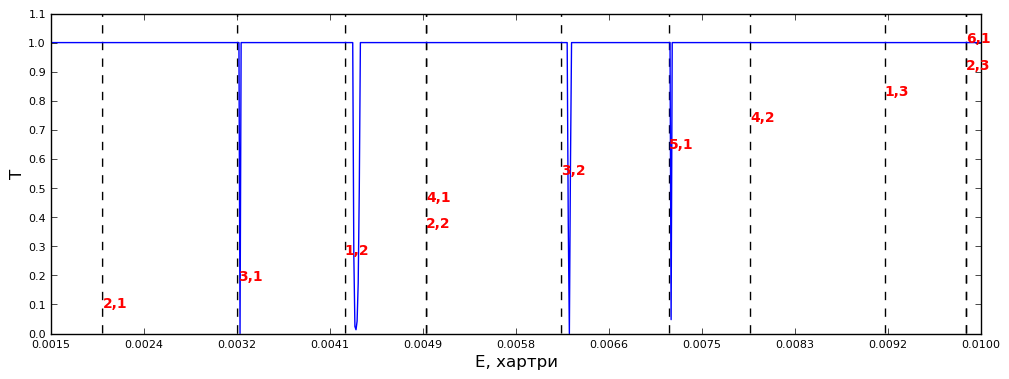
\includegraphics[width=0.8\textwidth]{transmission_all.png}
\caption{Зависимость коэффициента прохождения от энергии входящей волны. Вертикальные пунктирные линии — собственные энергии резонатора, парами чисел помечены номера соответствующих им собственных состояний.}
\end{figure}
\end{frame}

\begin{frame}[fragile]
\frametitle{Результаты: плотность вероятности в резонансной точке}
\begin{figure}
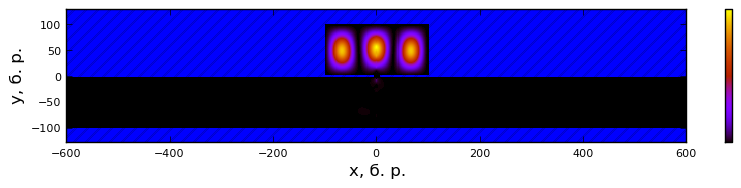
\includegraphics[width=0.8\textwidth]{pdensity_31_r.png}
\caption{Плотность вероятности в резонансной точке}
\end{figure}
\end{frame}

\begin{frame}[fragile]
\frametitle{Результаты: плотность вероятности в окрестности резонансной точки}
\begin{figure}
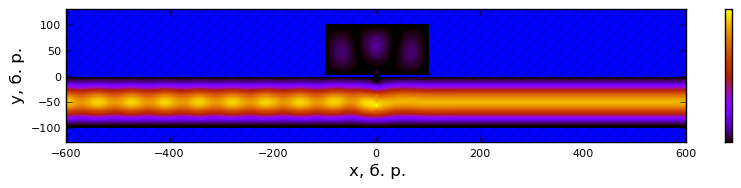
\includegraphics[width=0.8\textwidth]{pdensity_31_nr.png}
\caption{Плотность вероятности в небольшой окрестности резонансной точки}
\end{figure}
\end{frame}

\begin{frame}[fragile]
\frametitle{Результаты: коэффициент прохождения в окрестности резонанса}
\begin{figure}
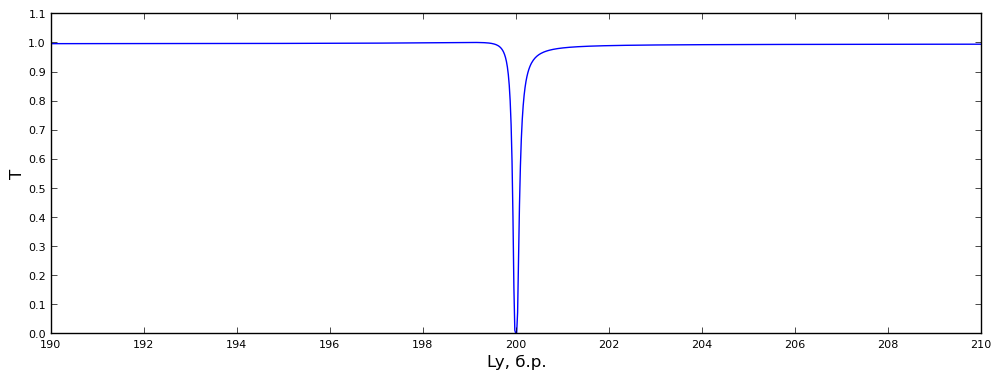
\includegraphics[width=0.8\textwidth]{transmission_size.png}
\caption{Зависимость коэффициента прохождения от геометрии резонатора}
\end{figure}
\end{frame}


% \begin{frame}[fragile]
% \frametitle{Проверка результатов}
% \begin{easylist}[itemize]
% # Все плохо
% ## Задача никем не решалась, не с чем сравнивать
% ## Не ясно, как решать численно
% \end{easylist}
% \end{frame}


\begin{frame}[fragile]
\frametitle{Дальнейшие вариации задачи}
\begin{easylist}[itemize]
# Двумерный волновод, квантовая точка внутри проводника
# Трехмерный волновод, квантовая точка внутри проводника
# Трехмерный волновод, тороидальный резонатор Гельмгольца
## Взаимодействие не точечное, но за счет симметрии может получиться что-то хорошее
# Полупрозрачная перегородка 
# Уравнение Дирака
## Учитывает релятивистские эффекты
# Магнитное поле
\end{easylist}
\end{frame}

\end{document}


% !!!!!!!
% \begin{comment}

% \begin{frame}[fragile]
% \frametitle{Расширение пространства: шкалы}
% \begin{easylist}[itemize]
% # $H$ — самосопряженный оператор, действующий в $\hilb{0}$ со скалярным произведением $\ip{\cdot}{\cdot}_0$
% # Резольвента: $R(z) = \frac{1}{H - z}$. Пусть $z_0 \in \rho(H)$ (произвольное), $Z_0 = R(z_0)$
% # Положительная шкала: для $k > 0$, определим $\hilb{k} = Z_0^k \hilb{0} = \{ Z_0^k \phi \mid \phi \in \hilb{0} \}$, «хорошие» функции
% ## $\dots \subseteq \hilb{k} \subseteq \hilb{k - 1} \subseteq \dots \subseteq \hilb{1} \subseteq \hilb{0}$
% ## В каждом $\hilb{k}$ определим скалярное произведение: $\ip{f}{g}_k = \ip{Z_0^{-k} f}{Z_0^{-k} g}_0$
% # Отрицательная шкала: для $k > 0$, определим $\hilb{-k}$ как пополнение пространства $\hilb{0}$ по норме $\|f \|_{-k} = \sup\limits_{u \in \hilb{k}} \frac{\ip{f}{u}_0}{\|u\|_j}$, «плохие» функции
% ## $\hilb{0} \subseteq \hilb{-1} \subseteq \dots \subseteq \hilb{-k} \subseteq \hilb{-k - 1} \subseteq \dots $
% \end{easylist}
% \end{frame}


% \begin{frame}[fragile]
% \frametitle{Расширение пространства: шкалы (продолжение)}
% \begin{easylist}[itemize]
% # Скалярное произведение $\ip{\cdot}{\cdot}_0: \hilb{0} \times \hilb{0} \to \bbC$ можно расширить до $\ip{\cdot}{\cdot}_E: \hilb{-k} \times \hilb{k} \to \bbC$
% \begin{align*}
% \ip{f}{g}_E &\eqdef \lim\limits_{n \to \infty} \ip{f_n}{u}_0 \\
% \ip{g}{f}_E &\eqdef \cconj{\ip{f}{g}}
% \end{align*}
% \end{easylist}
% \end{frame}


% \begin{frame}[fragile]
% \frametitle{Расширение пространства: предпонтрягинское пространство}
% \begin{easylist}[itemize]
% # Пусть $\psi$ — «плохой» элемент не из $\hilb{0}$ (в нашем случае производная функции Грина)
% ## $\psi \in \hilb{-m} \setminus \hilb{-m + 1}$ 
% # Хотим получить пространство $\mcP$ такое, что:
% ## Содержит элемент $\psi$
% ## Содержит как можно меньше «лишних» элементов $\hilb{-m} \setminus \hilb{0}$
% ## Содержит как можно больше элементов из $\hilb{0}$
% ## Скалярное произведение в $\mcP$ определено на всех парах элементов и расширяет исходное
% \end{easylist}
% \end{frame}


% \begin{frame}[fragile]
% \frametitle{Расширение пространства: предпонтрягинское пространство (продолжение)}
% \[
% \mathcal{P} = 
% \{ \varphi_m + \sum\limits_{i = -m}^{m - 1} c_i \psi_i \mid \varphi_m \in \hilb{m}, c_i \in \mathbb{C}\}
% \]
% , где $\psi_i = Z_0^{m + i} \psi$, то есть, $\psi_i \in \hilb{i}$.

% \begin{align*}
% \ip{f}{f'}_{\mcP}
% &= \ip{\varphi_m}{\varphi'_m}_E \\
% &+ \sum\limits_{i = -m}^{m - 1} \ip{c_i \psi_i}{\varphi'_m}_E + \sum\limits_{j = -m}^{m - 1} \ip{\varphi_m}{c_j' \psi_j}_E \\
% &+ \sum\limits_{i = -m}^{m - 1} \sum\limits_{j = -m}^{m - 1} \cconj{c_i} g_{ij} c_j'
% \end{align*}
% \end{frame}


% \begin{frame}[fragile]
% \frametitle{Расширение пространства: предпонтрягинское пространство (продолжение)}
% \begin{easylist}[itemize]
% # $g_{ij}$ — эрмитова матрица: $g_{ij} = \cconj{g_{ji}}$
% # Некоторые из элементов $g_{ij}$ могут быть корректно определены, если $\psi_i$ и $\psi_j$ совместны, в частности, когда $i + j \ge 0$
% # Для выполнения резольвентного тождества, необходимо $\mel{f}{R_0(z_0)}{g} = \cconj{\mel{g}{R_0(\cconj{z_0})}{f}}$, что означает
% $g_{i + 1, j} - g_{i, j + 1} = (z_0 - \cconj{z_0}) g_{i + 1, j + 1}$
% # Оставшиеся элементы (а это, как минимум, $g_{-m, -m}$) — свободные параметры, определяются из некоторых физических соображений (т.н. ренормализация)
% \end{easylist}
% \end{frame}


% \begin{frame}[fragile]
% \frametitle{Расширение пространства: понтрягинское пространство}
% Но в $\mcP$ все еще не все элементы $\hilb{0}$!

% Определим 
% \[
% \Pi = \{f = (\phi_f, \vb{p_f}, \vb{n_f}) \mid \phi_f \in \hilb{0}, \vb{p_f}, \vb{n_f} \in \mathbb{C}^m \}
% \]
% с индефинитным скалярным произведением
% \[
% \ip{f}{g}_\Pi =
% \ip{\phi_f}{\phi_g}_E +
% \cconj{\vb{p_f}} \vdot \vb{n_g} +
% \cconj{\vb{n_f}} \vdot \vb{p_g} + 
% \cconj{\vb{n_f}} \vdot \vb{g_{ij}} \vdot \vb{n_g}
% \]

% Вложим $\mathcal{P}$ в $\Pi$:
% \begin{align*}
% \varphi_m + \sum\limits_{i = -m}^{m - 1} c_i \psi_i \mapsto
% \big(
% & \varphi_m + \sum\limits_{i = 0}^{m - 1} c_i \psi_i, \\
% & \left[ \ip{\psi_i}{\varphi_m}_E + \sum\limits_{j = 0}^{m - 1} c_j g_{ij} \right]_{i = -1}^{-m}, \\
% & \left[ c_i \right]_{i = -1}^{-m}  \big)
% \end{align*}
% \end{frame}


% \begin{frame}[fragile]
% \frametitle{Расширение пространства: понтрягинское пространство (продолжение)}
% \begin{easylist}[itemize]
% # Вложение — плотное, пополнением $\mcP$ будет понтрягинское пространство $\Pi$
% # Операторы, ранее определенные на $\hilb{0}$, также замыкаются в $\Pi$
% \end{easylist}
% \end{frame}
% \end{comment}